
%%%%%%%%%%%%%%%%%%%%%%% paper_sem_web.tex %%%%%%%%%%%%%%%%%%%%%%%%%
%
% This is the LaTeX source for the instructions to authors using
% the LaTeX document class 'llncs.cls' for contributions to
% the Lecture Notes in Computer Sciences series.
% http://www.springer.com/lncs       Springer Heidelberg 2006/05/04
%
% It may be used as a template for your own input - copy it
% to a new file with a new name and use it as the basis
% for your article.
%
% NB: the document class 'llncs' has its own and detailed documentation, see
% ftp://ftp.springer.de/data/pubftp/pub/tex/latex/llncs/latex2e/llncsdoc.pdf
%
%%%%%%%%%%%%%%%%%%%%%%%%%%%%%%%%%%%%%%%%%%%%%%%%%%%%%%%%%%%%%%%%%%%


\documentclass[runningheads,a4paper]{llncs}
\usepackage[utf8x]{inputenc}
\usepackage{amssymb}
\setcounter{tocdepth}{3}
\usepackage{graphicx}

\usepackage{url}
\urldef{\mailsa}\path|{manuel.b.dudda, robert.c.brylka, frank.b.reichwein,}@student.hs-rm.de|    
\newcommand{\keywords}[1]{\par\addvspace\baselineskip
\noindent\keywordname\enspace\ignorespaces#1}

\begin{document}

\mainmatter  % start of an individual contribution

% first the title is needed
\title{Semantic Web Technologien:\\FIFA's Fu\ss ball-Weltmeisterschaft 2014 in Brasilien bekommt eine semantische Unterst\"utzung.}

% a short form should be given in case it is too long for the running head
\titlerunning{Semantic Web: Brasil WM 2014}

% the name(s) of the author(s) follow(s) next
%
% NB: Chinese authors should write their first names(s) in front of
% their surnames. This ensures that the names appear correctly in
% the running heads and the author index.
%
\author{Manuel Dudda%
\thanks{Herzlichen Dank, dass Du das Projekt im allein Gang auf die Beine gestellt hast und von uns nur verlangt hast, dass wir einmal die Hose runter lassen :-).}%
\and Robert Brylka\and Frank Reichwein}
%
\authorrunning{Brasil WM 2014 mit Semantic Web}
% (feature abused for this document to repeat the title also on left hand pages)

% the affiliations are given next; don't give your e-mail address
% unless you accept that it will be published
\institute{Hochschule RheinMain Informatik Master of Science \\
Fachbereich Design Informatik Medien \\
Campus Unter den Eichen 5
65195 Wiesbaden , Deutschland\\
\mailsa\\
\url{http://www.http://semanticwc.herokuapp.com}}

%
% NB: a more complex sample for affiliations and the mapping to the
% corresponding authors can be found in the file "llncs.dem"
% (search for the string "\mainmatter" where a contribution starts).
% "llncs.dem" accompanies the document class "llncs.cls".
%

\toctitle{Lecture Notes in Computer Science}
\tocauthor{Authors' Instructions}
\maketitle


\begin{abstract}
Große Sportereignisse haben schon immer große Menschenmaßen begeistert. So auch die Events die die Disziplin Fußball betreffen. Dieses Paper beschreibt ein Projekt, das sich als Ziel die Vorstellung der Ereignisse der diesjährigen Fußballweltmeisterschaft gesetzt hat. Der Fokus dieser Anwendung liegt auf der Aktualität der präsentierten Daten sowie einer auf die Mobilen-Endgeräte angepassten Repräsentation. Für die Vielfalt der präsentierten Daten sowie deren Richtigkeit sorgte eine Informationssynthese aus mehreren Quellen. Um die Informationen weitestgehend für automatische Weiterverarbeitung vorzubereiten wurden alle Daten um semantische Bedeutung aus gängigen Sport-Ontologien ergänzt.
\end{abstract}

\section{Pitch}

\section{Introduction}

\newpage
\section{Bestimmung der Informationsquellen}\label{infoQuell}

Die Fußballweltmeisterschaft ist allgemein ein belebtes Thema in der digitalen Welt. Um geeignete Quellen für die gesuchte Informationen zu finden wurde eine tiefgründige Recherche durchgeführt. Die unten aufgeführte Tabelle zeigt ein Ausschnitt aus der Zusammenstellung in der die geeigneten Quellen aufgeführt wurden. Wie man an der Zusammenstellung erkennen kann verfügen nicht alle Quellen über die gleiche Informationsfülle. Dabei ist die Open Football \cite{url_openfootball} Datenbank aufgrund der nicht aktuellen Informationen für weitere Verwendung uninteressant. Die Football Data \cite{url_footballdata} sowie die World Cup \cite{url_worldcup} Datenbank zeigen beide eine sehr gute Fülle an brauchbaren Informationen. Bei einer weiteren Recherche zu der Word Cup Datenbank wurde die offengelegte API gefunden die einen direkten Zugriff auf die offizielle Seite der FIFA ermöglicht. Wie die letzte Spalte der Zusammenstellung zu entnehmen ist, ist die offizielle Seite des Internationalen Fußballverbandes die beste Informationsquelle. Im Entschluss wurde die Word Cup API mit Anpassungen auf ein REST\footnote{\textbf{Re}presentational \textbf{S}tate \textbf{T}ransfer} JSON\footnote{\textbf{J}ava\textbf{S}cript \textbf{O}bject \textbf{N}otation} Server aufgesetzt. Das Ergebnis ist eine JSON Datei mit allen relevanten Informationen.

\begin{center}
%\begin{table}

\begin{tabular}{|l|c|c|c|c|c|}   \hline 
 & Football Data 	& Open Football 	& Footbal DB  &	World Cup  & FIFA  \\ \hline
References & \cite{url_footballdata} & \cite{url_openfootball} &  \cite{url_footballdb} &
 \cite{url_worldcup} & \cite{url_fifa} \\ \hline
 
Teams				& + & + & +	& + & +		\\ \hline
Gruppen				& - & + & -	& + & +		\\ \hline
Spiele				& + & + & -	& + & +		\\ \hline
Stadien				& + & + & -	& + & +		\\ \hline
Uhrzeiten			& + & + & -	& + & +		\\ \hline
Spieler				& + & + & - & - & +		\\ \hline
Spielergebnisse		& + & + & + & + & + 		\\ \hline
Torschützen/min		& +/+ & 	+/+ & - & + & +/+ 	\\ \hline
Schiedsrichter		& - & - & - & - & +		\\ \hline
Trainer				& - & - & - & - & +		\\ \hline
Spieltag 			& + & + & + & + & +		\\ \hline
Aktuell				& - & - & + & + & +  \\ \hline
Besucherzahl			& + & - & - & - & +		\\ \hline
			 
\end{tabular}
%\end{table}

%\label{tab:tab1} 

%\caption{Zusammenstellung der wichtigsten Informationsquellen}	
\end{center}


Eine wichtige Rolle bei der Wahl der API hat letztendlich auch der Finanzielleaspekt gespielt. Es gibt eine ganze Reihe an gut organisierten und stets aktuellen Datenbanken, die jedoch eine monatliche Gebühr mit sich tragen. Für dieses Projekt wurde jedoch eine Vereinbarung getroffen, rein Quelloffene Lösungen zu verwenden. Dadurch sind Finanziellabhängige Projekte direkt bei der Recherche ausgeschlossen worden. 
  
\newpage
\section{Ontologien}

\begin{figure}
\centering
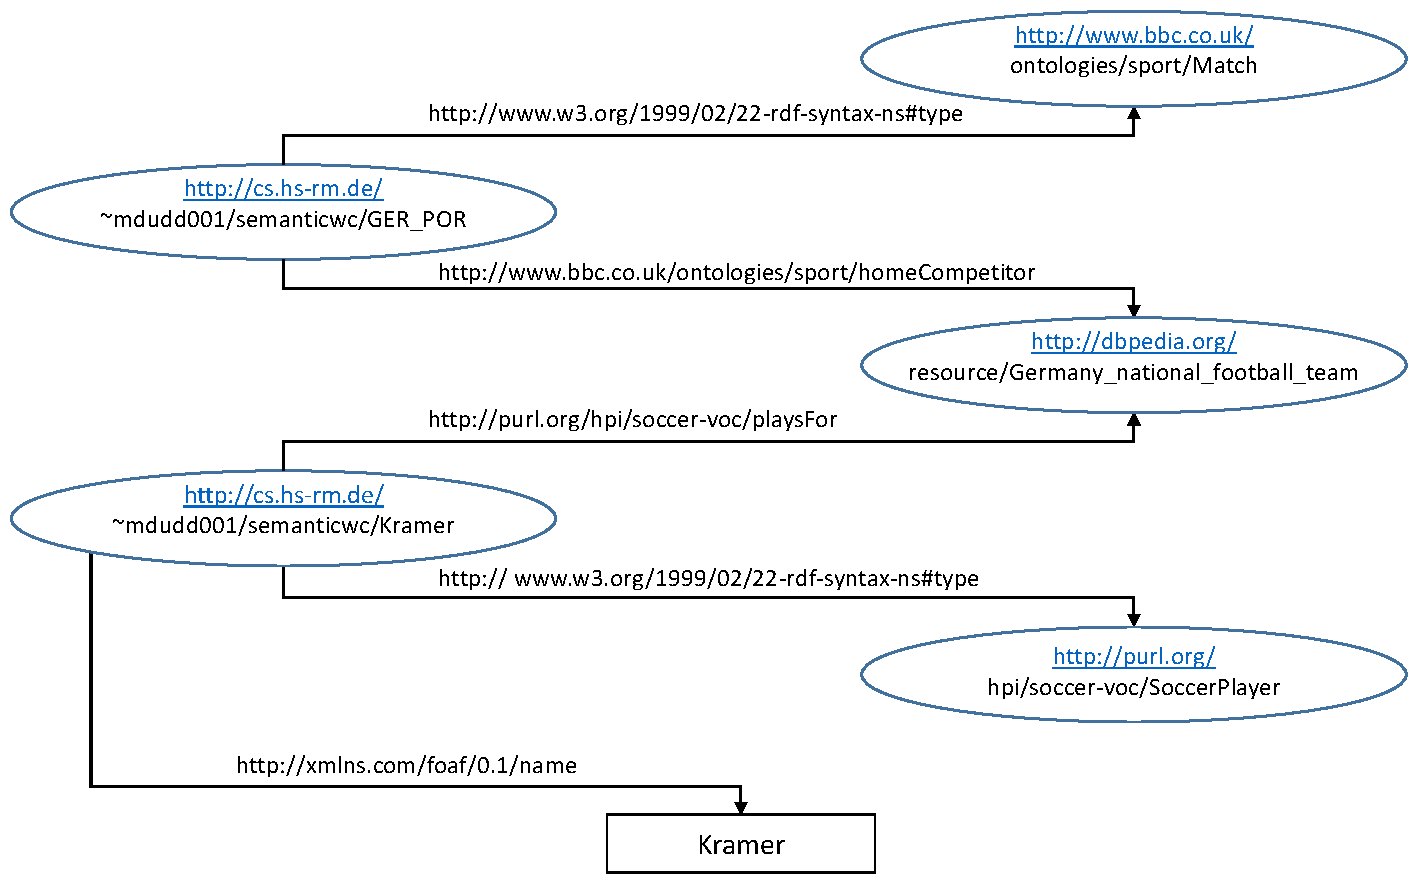
\includegraphics[height=7.2cm]{graph_manus}
\caption{Exemplarische Ausschnitt aus der RDF.}
\label{fig:example}
\end{figure}

\newpage
\section{Application // Implemetierung}


Bei der Wahl des Framework für diese Anwendung fiel die Entscheidung zu Gunsten von Ruby on Rails \footnote{http://www.rubyonrails.org/}. Dieses quelloffenes Web Application Framework bietet sehr gute Unterstützung bei Entwicklung von Semantik Web Applikationen um die RDF Datenbank oder den SPARQL Client zu nennen . Als Unterstützung für die Mobilen-Endgeräte, z.B. für den Swipe-Efect,  wurde die jQuery mobile\footnote{http://www.jquerymobile.com/} Bibliothek eingesetzt. 

\begin{figure}
\centering
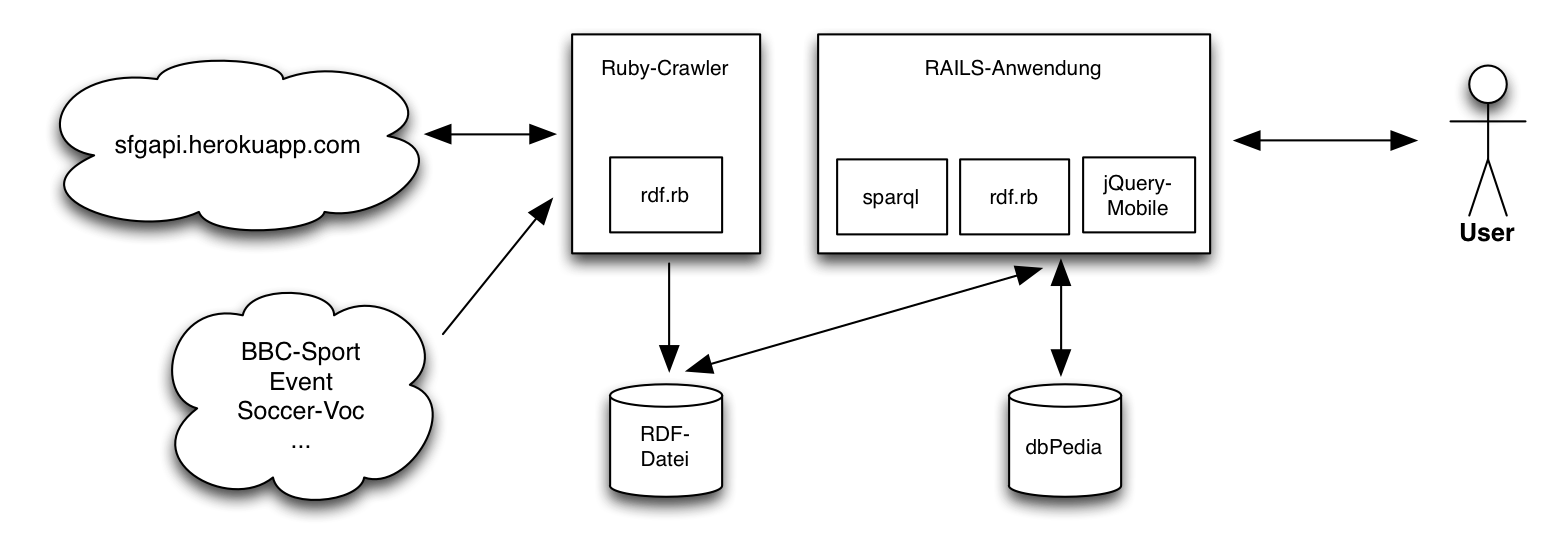
\includegraphics[height=4.2cm]{technik-stack}
\caption{Technik-stack.}
\label{fig:example}
\end{figure}

\begin{figure}
\centering
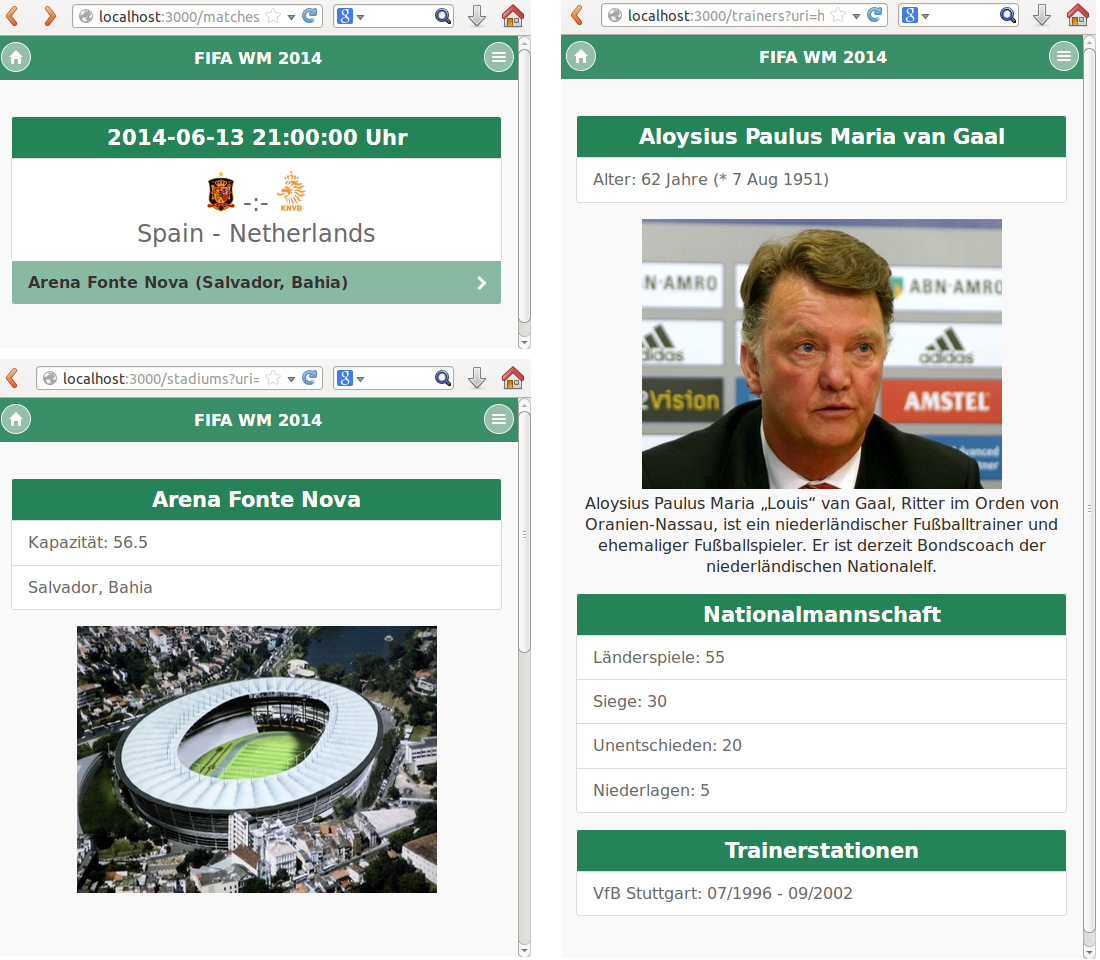
\includegraphics[height=8.2cm]{screenshots}
\caption{Screenshots der Anwendung. Abbildung oben links zeigt die }
\label{fig:screenshots}
\end{figure}

\newpage
\section{Zusammenfassung und Ausblick}

Im Rahmen dieses Projekts wurde eine Anwendung entwickelt, die alle wichtigen Informationen, zu der 2014 in Brasilien stattfindenden Fußball Weltmeisterschaft, bereithält. Als Informationsquelle dient hierbei die offizielle FIFA Webseite, die mit Daten aus der DPpedia ergänzt wurde. Die semantische Aufbereitung wurde mit Hilfe der BBC Sport sowie der Socker Voc Ontologie gestaltet.  

Unsere Anwendung bietet eine solide Grundlage für Weiterentwicklungen die nicht nur den Bereich Fußball betreffen. Bezogen auf die Fußballereignisse kann eine leichte Portierung auf die nächste Weltmeisterschaft oder Europameisterschaft stattfinden. Denkbar ist aber auch eine Abwandlung zur Informationspräsentation der Spiele der Bundesliga Mannschaften. 

\begin{thebibliography}{4}
\bibitem{url_bbc}BBC ONTOLOGIES,
Letzter Zugriff: 26. Juni 2014\\
\url{http://www.bbc.co.uk/ontologies}

\bibitem{url_jquery}jQuery mobile,
Letzter Zugriff: 26. Mai 2014\\
\url{https://demos.jquerymobile.com/1.4.2/}

\bibitem{url_smm}Semantic Media Mining,
Letzter Zugriff: 22. Juli 2014\\
\url{https://smm2013.blogspot.de/2012/11/soccer-voc.html}

\bibitem{url_dbpedia}DBpedia,
Letzter Zugriff: 22. Juli 2014\\
\url{http://http://dbpedia.org}

\bibitem{url_ruby}Ruby. Der beste Freund eines Programmierers,
Letzter Zugriff: 22. Juli 2014\\
\url{https://www.ruby-lang.org/de/}

\bibitem{url_footballdata}Scraping FIFA World Cup Data,
Letzte Zugriff: 12. Juli 2014\\
\url{https://github.com/footballdata/fifadata}

\bibitem{url_openfootball}Open Football,
Letzter Zugriff: 12. Juli 2014\\
\url{https://github.com/openfootball/world-cup}

\bibitem{url_footballdb}Footbal DB,
Letzter Zugriff: 12. Juli 2014\\
\url{http://footballdb.herokuapp.com/api/v1/}

\bibitem{url_worldcup}World Cup ... in JSON,
Letzter Zugriff: 12. Juli 2014\\
\url{http://www.http://worldcup.sfg.io/}

\bibitem{url_fifa}FIFA com,
Letzter Zugriff: 12. Juli 2014\\
\url{http://http://www.fifa.com/}

\end{thebibliography}


\section*{Appendix: Springer-Author Discount}

LNCS authors are entitled to a 33.3\% discount off all Springer
publications. Before placing an order, the author should send an email, 
giving full details of his or her Springer publication,
to \url{orders-HD-individuals@springer.com} to obtain a so-called token. This token is a
number, which must be entered when placing an order via the Internet, in
order to obtain the discount.

\section{Checklist of Items to be Sent to Volume Editors}
Here is a checklist of everything the volume editor requires from you:


\begin{itemize}
\settowidth{\leftmargin}{{\Large$\square$}}\advance\leftmargin\labelsep
\itemsep8pt\relax
\renewcommand\labelitemi{{\lower1.5pt\hbox{\Large$\square$}}}

\item The final \LaTeX{} source files
\item A final PDF file
\item A copyright form, signed by one author on behalf of all of the
authors of the paper.
\item A readme giving the name and email address of the
corresponding author.
\end{itemize}
\end{document}
